\documentclass[tikz,border=12pt]{standalone}
\usepackage[T1]{fontenc}
\usepackage{mathpazo}
\usepackage{amsmath,amssymb}
\usetikzlibrary{arrows.meta, positioning, calc, fit, decorations.pathreplacing}

\definecolor{stblue}{HTML}{7B97AD}
\definecolor{rwgold}{HTML}{B8995E}
\definecolor{sage}{HTML}{7A9A7E}
\definecolor{dkbrown}{HTML}{3D3530}
\definecolor{wmgray}{HTML}{7B7067}
\definecolor{cream}{HTML}{F9F6F0}
\definecolor{border}{HTML}{D4C9B8}
\definecolor{terracotta}{HTML}{C47A6A}
\definecolor{lavender}{HTML}{907EA0}

\begin{document}
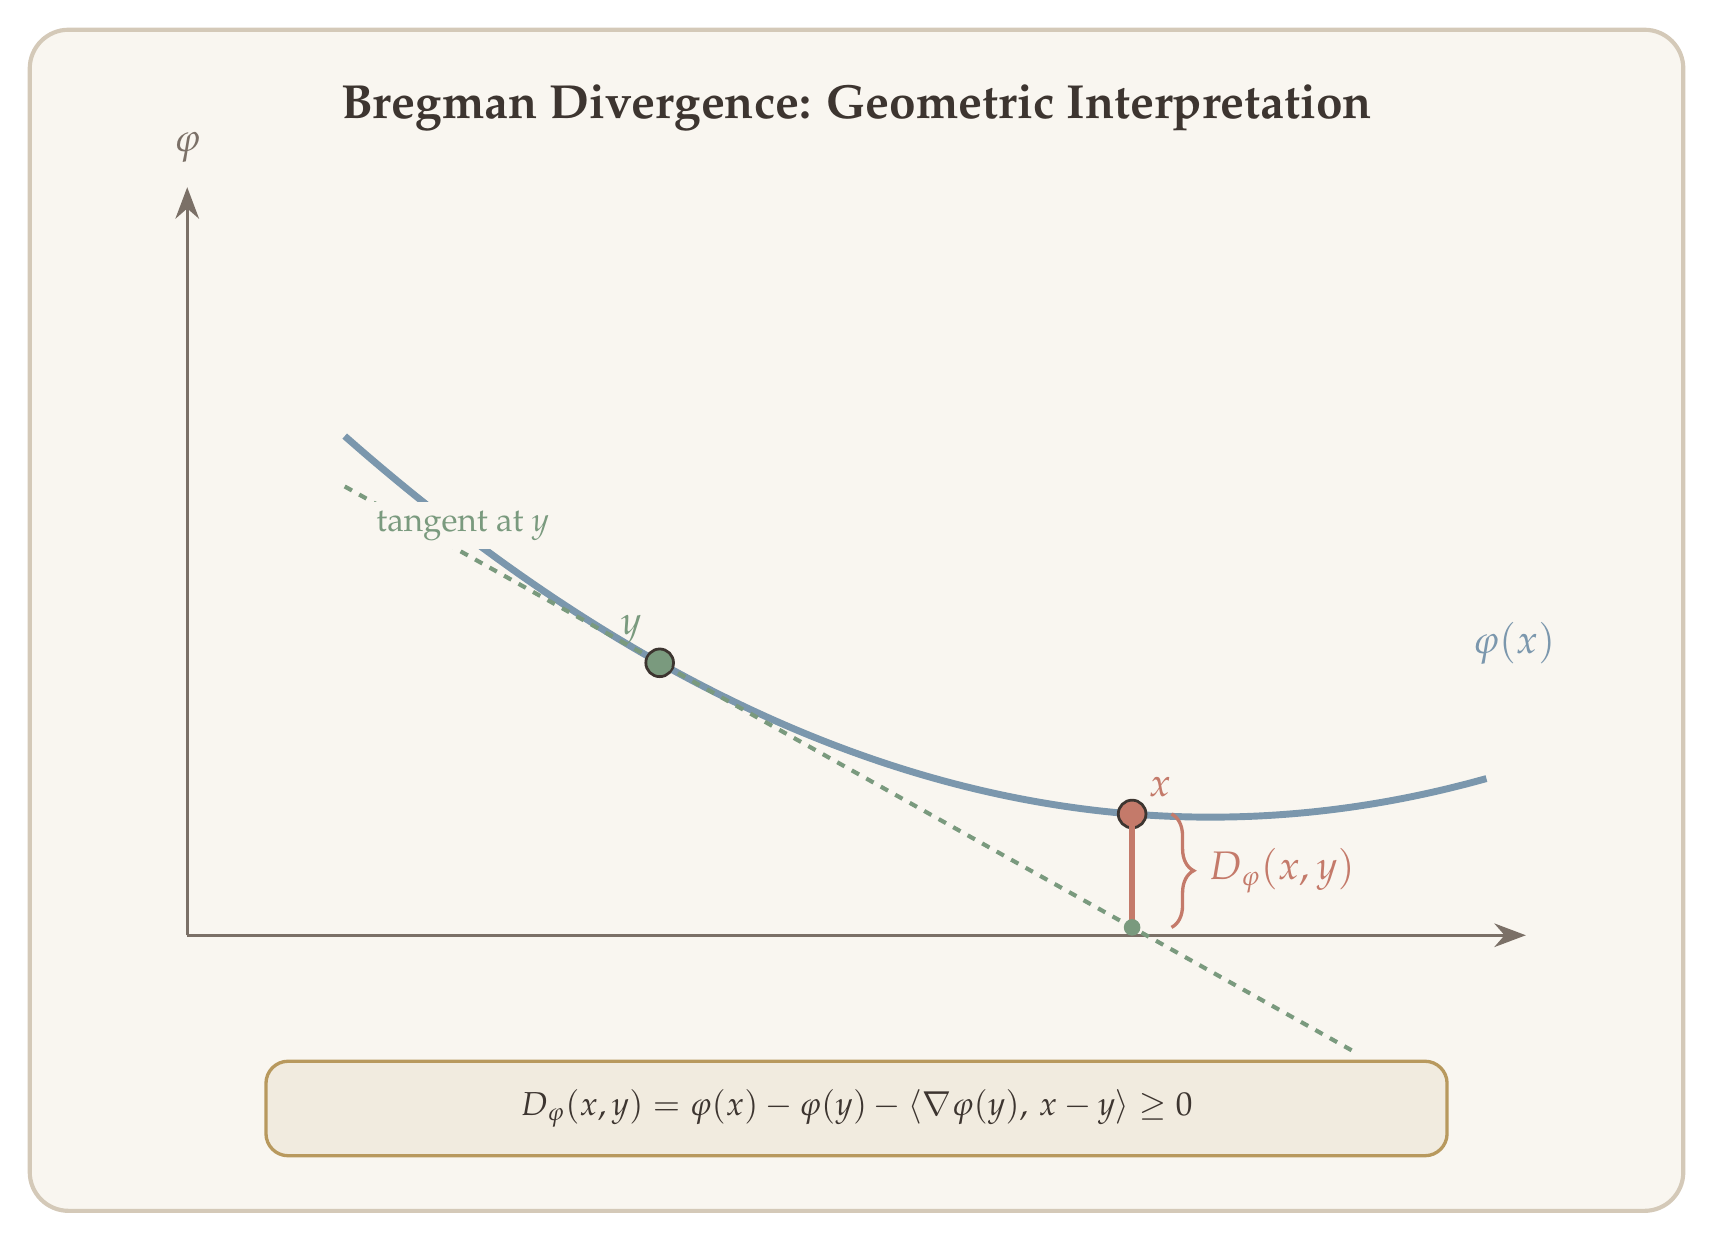
\begin{tikzpicture}[>={Stealth[length=4mm, width=3mm]}]

% Background
\fill[cream, rounded corners=14pt] (-1,-2) rectangle (20,13);
\draw[border, line width=1.5pt, rounded corners=14pt] (-1,-2) rectangle (20,13);

% Title
\node[text=dkbrown, font=\LARGE\bfseries] at (9.5,12.0) {Bregman Divergence: Geometric Interpretation};

% Axes
\draw[wmgray, line width=1pt, ->] (1.0,1.5) -- (18.0,1.5);
\draw[wmgray, line width=1pt, ->] (1.0,1.5) -- (1.0,11.0);
\node[text=wmgray, font=\Large] at (1.0,11.5) {$\varphi$};

% Convex function: phi(x) = 0.04*(x-14)^2 + 3.0
% Plotted directly in canvas coordinates (x is canvas x)
\draw[stblue, line width=2.5pt, smooth, samples=60, domain=3:17.5]
  plot (\x, {0.04*(\x-14)*(\x-14) + 3.0});
\node[text=stblue, font=\Large, right] at (17.2,5.2) {$\varphi(x)$};

% Point y at canvas x=7: phi(7) = 0.04*49 + 3 = 4.96
\fill[sage] (7,4.96) circle (5pt);
\draw[dkbrown, line width=1pt] (7,4.96) circle (5pt);
\node[text=sage, font=\Large\bfseries, above left=4pt] at (7,4.96) {$y$};

% Tangent line at y: phi'(7) = 0.08*(7-14) = -0.56
% line(t) = 4.96 - 0.56*(t-7) = 8.88 - 0.56*t
\draw[sage, line width=1.5pt, dashed, domain=3:15.8]
  plot (\x, {8.88 - 0.56*\x});

% Point x at canvas x=13: phi(13) = 0.04*1 + 3 = 3.04
\fill[terracotta] (13,3.04) circle (5pt);
\draw[dkbrown, line width=1pt] (13,3.04) circle (5pt);
\node[text=terracotta, font=\Large\bfseries, above right=4pt] at (13,3.04) {$x$};

% Tangent value at x=13: line(13) = 8.88 - 7.28 = 1.6
% D_phi(x,y) = phi(x) - tangent(x) = 3.04 - 1.6 = 1.44

% Vertical line showing the gap D_phi
\draw[terracotta, line width=2pt] (13,1.6) -- (13,3.04);
\fill[sage] (13,1.6) circle (3pt);

% Brace annotation for D_phi
\draw[terracotta, line width=1.2pt, decorate, decoration={brace, amplitude=8pt, mirror}]
  (13.5,1.6) -- (13.5,3.04);
\node[text=terracotta, font=\Large\bfseries, right=10pt] at (13.5,2.32) {$D_\varphi(x, y)$};

% Label for tangent line — placed on the left portion, away from the brace
\node[text=sage, font=\large, fill=cream, inner sep=3pt, above] at (4.5,6.4)
  {tangent at $y$};

% Formula box at bottom
\fill[rwgold!20, rounded corners=8pt] (2.0,-1.3) rectangle (17.0,-0.1);
\draw[rwgold, line width=1.2pt, rounded corners=8pt] (2.0,-1.3) rectangle (17.0,-0.1);
\node[text=dkbrown, font=\large] at (9.5,-0.7)
  {$D_\varphi(x, y) = \varphi(x) - \varphi(y) - \langle\nabla\varphi(y),\, x - y\rangle \geq 0$};

\end{tikzpicture}
\end{document}
